\chapter{Offuscamento}

In questa capitolo si ha l'obiettivo di ingannare i tool di figerprinting, portandoli ad un risultato errato. Più precisamente, si ha lo scopo di modificare parametri di Kali per ottenere il riconoscimento di Windows.
\\
Non essendo Windows 11 presente nel database di Nmap e non potendo quindi essere un risultato del fingerprinting, si cercherà di portare i tool all'individuazione della sua versione precedente, ovvero Windows 10.

\section{Algoritmo utilizzato da Nmap}
Prima di procedere occorre precisare il funzionamento dell'algoritmo di Nmap per il riconoscimento dei sistemi operativi. Questo avviene secondo un meccanismo di punteggi che viene dato ad ogni test effettuato, specificato nella prima entry del database. I test che non ottengono alcun risultato utile non vengono conteggiati nel totale dei punti.
A questo punto, vi sono due possibili situazioni:
\begin{itemize}
	\item Se i risultati dei test combaciano perfettamente con quelli di una entry del database, allora quella verrà mostrata come risultato finale,
	\item Se i risultati dei test non coincidono con nessun sistema operativo, allora verranno calcolati i punti di ogni test soddisfatti per ogni sistema; quello con cui è stato realizzato un numero maggiore di punti sarà quello mostrato.
\end{itemize}

Segue l'elenco di test con il relativo punteggio:

\begin{lstlisting}[caption={Punteggi che Nmap attrribuisce ad ogni test}]
	MatchPoints
	SEQ(SP=25%GCD=75%ISR=25%TI=100%CI=50%II=100%SS=80%TS=100)
	OPS(O1=20%O2=20%O3=20%O4=20%O5=20%O6=20)
	WIN(W1=15%W2=15%W3=15%W4=15%W5=15%W6=15)
	ECN(R=100%DF=20%T=15%TG=15%W=15%O=15%CC=100%Q=20)
	T1(R=100%DF=20%T=15%TG=15%S=20%A=20%F=30%RD=20%Q=20)
	T2(R=80%DF=20%T=15%TG=15%W=25%S=20%A=20%F=30%O=10%RD=20%Q=20)
	T3(R=80%DF=20%T=15%TG=15%W=25%S=20%A=20%F=30%O=10%RD=20%Q=20)
	T4(R=100%DF=20%T=15%TG=15%W=25%S=20%A=20%F=30%O=10%RD=20%Q=20)
	T5(R=100%DF=20%T=15%TG=15%W=25%S=20%A=20%F=30%O=10%RD=20%Q=20)
	T6(R=100%DF=20%T=15%TG=15%W=25%S=20%A=20%F=30%O=10%RD=20%Q=20)
	T7(R=80%DF=20%T=15%TG=15%W=25%S=20%A=20%F=30%O=10%RD=20%Q=20)
	U1(R=50%DF=20%T=15%TG=15%IPL=100%UN=100%RIPL=100%RID=100%RIPCK=100%RUCK=100%RUD=100)
	IE(R=50%DFI=40%T=15%TG=15%CD=100)
\end{lstlisting}


\section{Modifiche al file sysctl.conf}
Per ottenere un sistema operativo differente, occorre modificare alcuni parametri del file sysctl.conf in modo da ottenere i valori di Windows.
La prima modifica riguarda il campo del TTL; variarlo da 64 a 128 consente di ingannate il test TG. La modifica vale per tutti i pacchetti che verranno inviati, quindi questo consente di spostare un grande quantità di punti a favore del riconoscimento di Windows, essendo il test ripetuto per molti pacchetti.

\begin{lstlisting}[caption={Modifica al campo TTL nel file sysctl.conf}]
	net.ipv4.ip_default_ttl=128
\end{lstlisting}

Un'ulteriore modifica può essere effettuata per quanto riguarda il flag ECN, la cui differenza è stata spiegata nel capitolo precedente. Questo riguarda i test della quarta riga, in cui quello specifico per la notifica esplicita di congestione ha un valore di 100 punti.

\begin{lstlisting}[caption={Modifica al campo ECN nel file sysctl.conf}]
	net.ipv4.tcp_ecn=0
\end{lstlisting} 

Il valore 0 significa che l'host non può accettare nè inizializzare l'utilizzo del flag ECN. Il comportamento in risposta a determinati pacchetti "patologici" è ora simile a quello di Windows.

Si può inoltre procedere modificando il valore della Windows Size massima, causando di conseguenza un cambiamento del valore del Window Scaling Factor, da 7 a 8. 
La riga scritta nel file è la seguente:

\begin{lstlisting}[caption={Modifica alla Windows Size massima nel file sysctl.conf}]
	net.core.rmem_max = 8388608
\end{lstlisting}

Questa modifica, presa singolarmente, non influenza il risultato del fingerprinting in quanto questo campo è contenuto all'interno delle TCP options, che vengono valutate in maniera aggregata. Servono quindi ulteriori modifiche che verranno illustrate successivamente.

\section{Modifiche tramite nftables}
La modifica dei pacchetti in uscita dall'host di cui si vuole effettuare il fingerprinting tramite nftables consente il cambiamento del comportamento solo in determinate situazioni; di particolare interesse sono quelle riguardanti i probe di Nmap.
\\
La differenza mostrata alla tabella \ref{tab:code} è oggetto di uno dei test effettuati da Nmap. Quest'ultimo, infatti, invia un pacchetto \textit{echo request} con campo \textit{code} impostato a 9, e valuta la risposta ricevuta.
Questa dovrebbe essere zero nel caso di un \textit{echo reply}, ma questo comportamento è in realtà dipendente dal sistema operativo in utilizzo.
Modificare i pacchetti echo reply in uscita per modificare il campo code nel caso questo sia 9 varia il risultato del test effettuato da Nmap. L'alto valore in termini di punteggio che questo test ha rende questa modifica molto importante ai fini del fingerprinting.\\
Il comando dato per ottenere questo comportamento è nel file nftables.conf, nella tabella output.

\begin{lstlisting}[caption={Modifica del campo code in caso di test Nmap}, label=codice_icmp]
	icmp type 0 icmp code 9 icmp code set 0
\end{lstlisting}

Si vuole inoltre modificare il valore della Window Size; anche in questo caso, il nuovo valore impostato dovrà rispecchiare il comportamento di Windows.

\begin{lstlisting}[caption={Modifica della Window Size}]
	tcp window != 0x2000 tcp window set 0x2000 counter name conta_window
\end{lstlisting}

Attuando tutte le modifiche elencate fino a questo punto, l'output di Nmap risulta essere il seguente:

\begin{figure}[h]
	\centering
	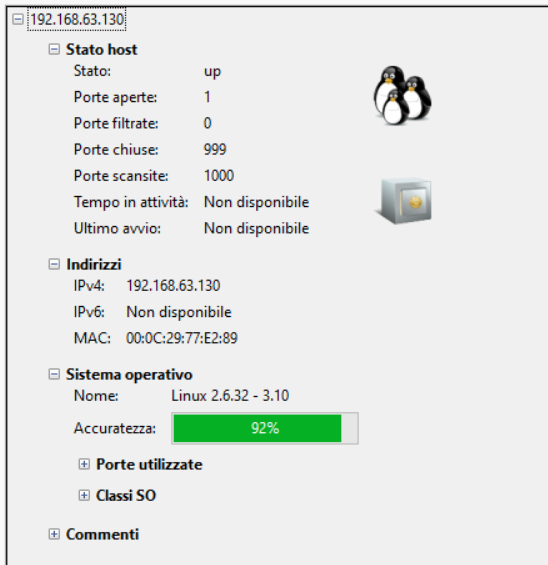
\includegraphics[scale=0.85]{figures/primo_nmap.png}
	\caption{Risultato di Nmap}
	\label{primo_nmap}
\end{figure}

Come si può evincere dall'immagine, viene riconosciuta una versione di Linux non corrispondente a quella attualmente in uso.
Visionando l'elenco completo dei test che vengono effettuati, si può notare che questi vengono preceduti da un port scanning, una procedura che ha l'obiettivo di esaminare l'apertura o meno di determinate porte dell'host.
Questa è fondamentale ai fini del fingerprinting perché l'individuazione di porte aperte o chiuse permette di effettuare test differenti, in grado di massimizzare il numero di informazioni ricavabili dalle risposte. Di default, Nmap scansiona 1000 porte.
\\
Nel risultato appena mostrato si può osservare come il tool abbia rilevato una sola porta aperta (la porta 80, su cui è attivo il server Apache) e 999 porte chiuse. I test eseguiti su quelle porte influenzano il risultato finale del fingerprinting, pertanto la possibilità di poterli escludere renderebbe molto più complessa l'individuazione del sistema operativo.
Per poter realizzare quanto descritto, occorre che l'host rifiuti tutti i pacchetti ricevuti che non abbiano come porta destinazione 80 (Well-Known port corrispondente ad HTTP).
\\
Si procede quindi inserendo una semplice regola nella tabella input delle nftables:

\begin{lstlisting}[caption={Regola per il blocco di tutti i pacchetti ricevuti non diretti alla porta 80}]
	tcp dport != 80 drop
\end{lstlisting}

Con l'utilizzo di questa regola, tutte le porte che prima risultavano \textit{chiuse} ora risultano \textit{filtrate}; la mancanza di test per pacchetti inviati alle porte filtrate influenza pesantemente il risultato del fingerprinting.

\begin{figure}[H]
	\centering
	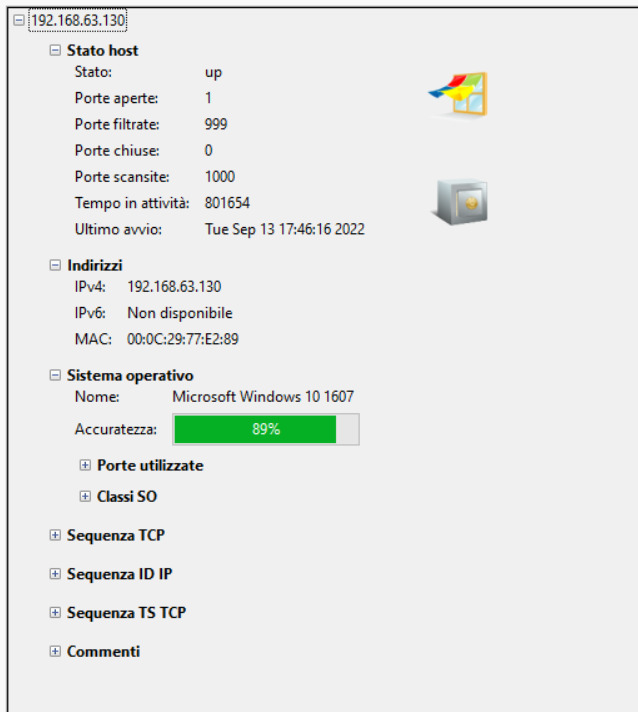
\includegraphics[scale=0.85]{figures/windows_nmap.png}
	\caption{Risultato di Nmap dopo il filtraggio dei pacchetti non diretti alla porta 80}
	\label{windows_nmap}
\end{figure}

Si tratta di un fingerprinting che Nmap definisce "aggressivo", dovuto al fatto che parecchi test non è stato possibile eseguirli; anche per questa ragione la percentuale di sicurezza di Nmap è 89\%, un valore elevato ma che testimonia l'assenza di una certezza assoluta.

\section{Offuscamento da fingerprinting passivo}
Le tecniche seguite per ingannare i tool di fingerprinting passivo non presentano numerose differenze rispetto alle precedenti; vi è però da considerare il fatto che i pacchetti analizzati non sono ricevuti in risposta a determinati probe.
Questo rende alcune regole impostate precedentemente non più funzionanti, come ad esempio la \ref{codice_icmp}; in questo caso, infatti, l'host non riceve alcun pacchetto echo request con campo code impostato a 9.





